%!TEX root = ../main.tex
\section{Introduction}
\label{sec:intro}

%\subsection{Large Language Models: Opportunities and Risks}

%\stitle{Large Language Models: Opportunities and Risks.}
The rise of \textbf{Large Language Models (LLMs)} has unlocked transformative {\bf opportunities} across diverse domains, including natural language processing, data analysis, and creative design, among many others. By enabling interaction with complex systems through intuitive natural language queries, LLMs democratize access to knowledge and data, allowing users to obtain valuable information quickly and cost-effectively without requiring specialized expertise or manual data processing. This accessibility has driven widespread adoption across industries such as healthcare, finance, and customer service, empowering both professionals and non-experts to extract insights and make informed decisions with ease. By reshaping traditional workflows, LLMs have the potential to significantly enhance productivity and decision-making across a wide range of applications.


However, alongside these opportunities, significant {\bf risks of LLMs} (or more generally, generative AI) have emerged. The phenomenon of {\em hallucinations}, \ie the generation of inaccurate or misleading information, poses a serious challenge to trust in LLM outputs. By 2023, analysts estimated that chatbots hallucinate as much as 27\% of the time\footnote{\url{https://www.nytimes.com/2023/11/06/technology/chatbots-hallucination-rates.html}}, and factual errors were present in 46\% of generated texts~\cite{de2023evaluation}, underscoring the prevalence of this issue.
These inaccuracies can negatively impact various aspects, including decision-making, the spread of misinformation, privacy violations, and potential legal liabilities. %Decisions based on erroneous information can have profound consequences, affecting not only individual organizations but also society at large.

%\subsection{Towards Trustworthy QA with LLMs: Efforts and Challenges}

%\textbf{Towards Trustworthy QA with LLMs.}
Developing \textbf{trustworthy solutions for question answering} is a priority for both academia and industry, with efforts focused on improving accuracy, reducing biases, and aligning models with human values. Companies like OpenAI and Google enhance model reliability through advanced training and Responsible AI principles\footnote{\url{https://openai.com/safety/}}. Initiatives like the Partnership on AI and collaborations by the AI Ethics Lab promote ethical guidelines and accountability in AI development\footnote{\url{https://aiethicslab.com/}}. However, challenges remain due to the probabilistic and generative nature of LLMs, which leads to unpredictability in outputs. While current efforts are valuable, they are insufficient to fully address issues such as inaccuracies, biases, and lack of explainability. More robust systems are needed, especially in high-stakes applications like data analysis over multimodal data, where trustworthiness is critical.


% The academic and industrial communities recognize the critical importance of addressing the challenges posed by LLMs on trustworthy AI, which underscores the necessity for collaborative efforts to develop LLM-based tools that are reliable, accurate, and aligned with human values.

% Efforts to promote trustworthy and responsible LLMs encompass industry, academia, and non-profit organizations. Model providers like OpenAI and Google enhance the factual accuracy of their systems and reduce biases through advanced model training\footnote{\url{https://openai.com/safety/}} and the implementation of Responsible AI Principles\footnote{\url{https://ai.google/responsibility/principles/}}.
% Initiatives such as the Partnership on AI play a pivotal role in establishing ethical guidelines and frameworks that ensure accountability in AI development\footnote{\url{https://partnershiponai.org/}}. This organization brings together diverse stakeholders to promote best practices in AI governance. Similarly, collaborative research efforts led by the AI Ethics Lab\footnote{\url{https://aiethicslab.com/}} foster partnerships between academia and industry to tackle pressing challenges in AI ethics and safety.
% Numerous researchers and practitioners are actively engaged in this work, reflecting a collective commitment to advancing responsible AI and ensuring that these technologies align with societal values. 
% % \textcolor{blue}{Do we need to mention RAG here?}

% Despite these promising efforts, significant challenges remain in developing fully trustworthy and reliable LLM-based systems. LLMs are probabilistic in nature, which inherently introduces a degree of unpredictability and uncontrollability in their outputs. The current efforts, while valuable, are not yet sufficient to fully address issues such as inaccuracies, persistent biases, and the difficulty of achieving explainability in generated output. More comprehensive systems are needed to tackle these challenges in specific applications, such as QA, where trustworthiness is crucial.


%\stitle{\sys: Trustworthy QA and Verification Using RAG over Multimodal Data Lakes.}
%

In this paper, we present \sys~\cite{symphony,verifai}, a system designed for trustworthy question answering and data analysis over multimodal data lakes. 
%\sys leverages Retrieval-Augmented Generation (RAG) to retrieve relevant external data from these data lakes, enhancing both the {\bf reasoning} and {\bf verification} processes. %Notably, the data lakes used for reasoning and verification may differ, allowing for tailored approaches to each phase.
%
Given a multimodal data lake $L$ and a natural language question $Q$ requiring factual or objective answers, the task of {\em reasoning} involves generating an answer to $Q$ by retrieving relevant data from $L$ and applying various reasoning tools such LLMs, RDBMSs, or graph databases.
%
Additionally, if an answer $A$ is provided—whether from humans or LLMs (possibly enhanced with RAG)—the task of {\em verification} is to assess the correctness of $A$ for $Q$, using the data lake $L$ (either a public data lake or a private/enterprise data lake) to ensure factual accuracy and reliability.


%the {\bf problem} that \sys tackles is to retrieve relevant data (\eg text, image, tables) from the data lake that can either help 


%\stitle{problem.}Given a multi-modal query \( Q \), which may consist of natural %language text and/or visual data (e.g., \( Q = (T, V) \), where \( T \) represents the text and \( V \) represents visual data, such as an image), the system first retrieves a relevant set of data items \( D \subseteq L \) from a multi-modal data lake \( L \). The data lake \( L \) contains various types of data, including text, images, and tables. After retrieving the relevant data \( D \), the system applies reasoning, often leveraging large language models, to generate an answer \( A \).

%To ensure the answer’s accuracy and relevance, a verification process is conducted by cross-referencing the generated answer \( A \) with the relevant data \( D \). This verification is formalized as:
%\(
%\text{verify}(A, x) \to \{0, 1, 2\}, \quad \forall x \in D
%\)
%Here, each data instance \( x \in D \) is evaluated against the generated answer \( A \), with the result being a ternary value: 0 indicates that the answer is verified, 1 indicates it is refuted, and 2 indicates that the data instance is not related to the answer. This verification process ensures that the generated answer is consistent with the multi-modal data \( D \), thereby enhancing the robustness and reliability of the system's response.\yang{For Q1 and Q5}

%\sys enhances the reliability and accuracy of generated answers through two core processes: \textbf{reasoning} and \textbf{verification}, both of which are supported by \textbf{multimodal data lakes}, which provide a diverse and reliable foundation of external information across various modalities, including text and tables.  By leveraging Retrieval-Augmented Generation (RAG), \sys retrieves relevant external data from the data lakes and integrates it into the reasoning and verification phases, ensuring that the system does not rely solely on internal model knowledge. Instead, it grounds its outputs in trustworthy, cross-modal sources for more accurate and reliable answers.


As illustrated in Figure~\ref{fig:symphony}, \sys comprises three core modules: 
(1) \discovery operates over multimodal data lakes and serves as the retrieval module; 
(2) \reason formulates answers to natural language questions using retrieved information and various tools; and 
(3) \verify assesses the correctness of provided answers utilizing LLMs and multimodal data lakes.
%
% Collectively, these modules work in harmony to ensure that \sys's responses are both accurate and grounded in reliable sources.

% {\em (1) Data Discovery over Multimodal Data Lakes:} 
% As the core module in \sys, multimodal data lakes house diverse data types, like text and tables, to support efficient retrieval for reasoning (question answering) and verification (response validation). Given a query, \sys effectively locates relevant information through three strategies: 
% 	(a) combining word-level and embedding-based similarity search for balanced speed and accuracy; 
% 	(b) Modal-agnostic Representation to unify data types in a shared space, facilitating effective cross-modal retrieval; and 
% 	(c) Modal-specific Representation with encoders tailored to each data type. While text and image representations are well-developed, structured table representation remains challenging due to the need to capture relationships across rows and columns. 
% Additionally, a human-in-the-loop system may iteratively refine results through feedback, improving retrieval relevance. %(Section~\ref{sec:learning})
% % The data lakes serve as the core module, providing a repository of diverse data types, including text and tables, which form the basis for effective information retrieval. To quickly and accurately extract relevant information for reasoning (based on the question) or verification (based on the generated answer), a key challenge lies in developing robust cross-modal representation learning strategies. \textcolor{blue}{lack of a clear description about what we do in this module.} This challenge is particularly significant for table representation learning, which requires specialized methods to encode structured data formats. Our approaches to cross-modal and table representation learning are detailed in Section~\ref{sec:learning}.

% {\em (2) RAG-based Reasoning:} 
% %During the reasoning phase, \sys retrieves relevant information from the multimodal data lakes. %By feeding external data and the question together into the LLM,  \sys ensures that its generated answers are grounded in reliable and diverse data sources rather than purely relying on internal model parameters. This process substantially enhances both the accuracy and reliability of the answers. 
% \sys utilizes a question decomposition strategy that breaks down queries into sub-questions, each of which can be addressed by a single data source and potentially different tools (e.g., LLMs, DBMSs, or BLIP). Furthermore, we propose optimization strategies to enhance reasoning efficiency and precision by striking a balance between speed and accuracy.
% %(Section~\ref{sec:reasoning})

% {\em (3) RAG-based Verification:}
% Even with RAG-based reasoning, errors may still occur due to the probabilistic nature of generative models, \eg the generated answer may include information not covered by the retrieved data, leading to inaccuracies. To address this, \sys includes an optional but valuable RAG-powered verification module. This module is not mandatory for every query, and users can choose to apply verification based on the complexity of the question or the reliability of the retrieved data.
% %
% After generating an answer, \sys retrieves additional relevant data from trusted sources to verify the output’s correctness and consistency. By incorporating private or enterprise data lakes, \sys ensures that the generated answers align with the knowledge base, policies, and standards of users or organizations. While public data lakes can also be used for verification, the focus on private data lakes arises from their ability to provide specialized, domain-specific content that enhances the relevance and precision of the verification process.

\begin{figure}[t!]
\begin{center}
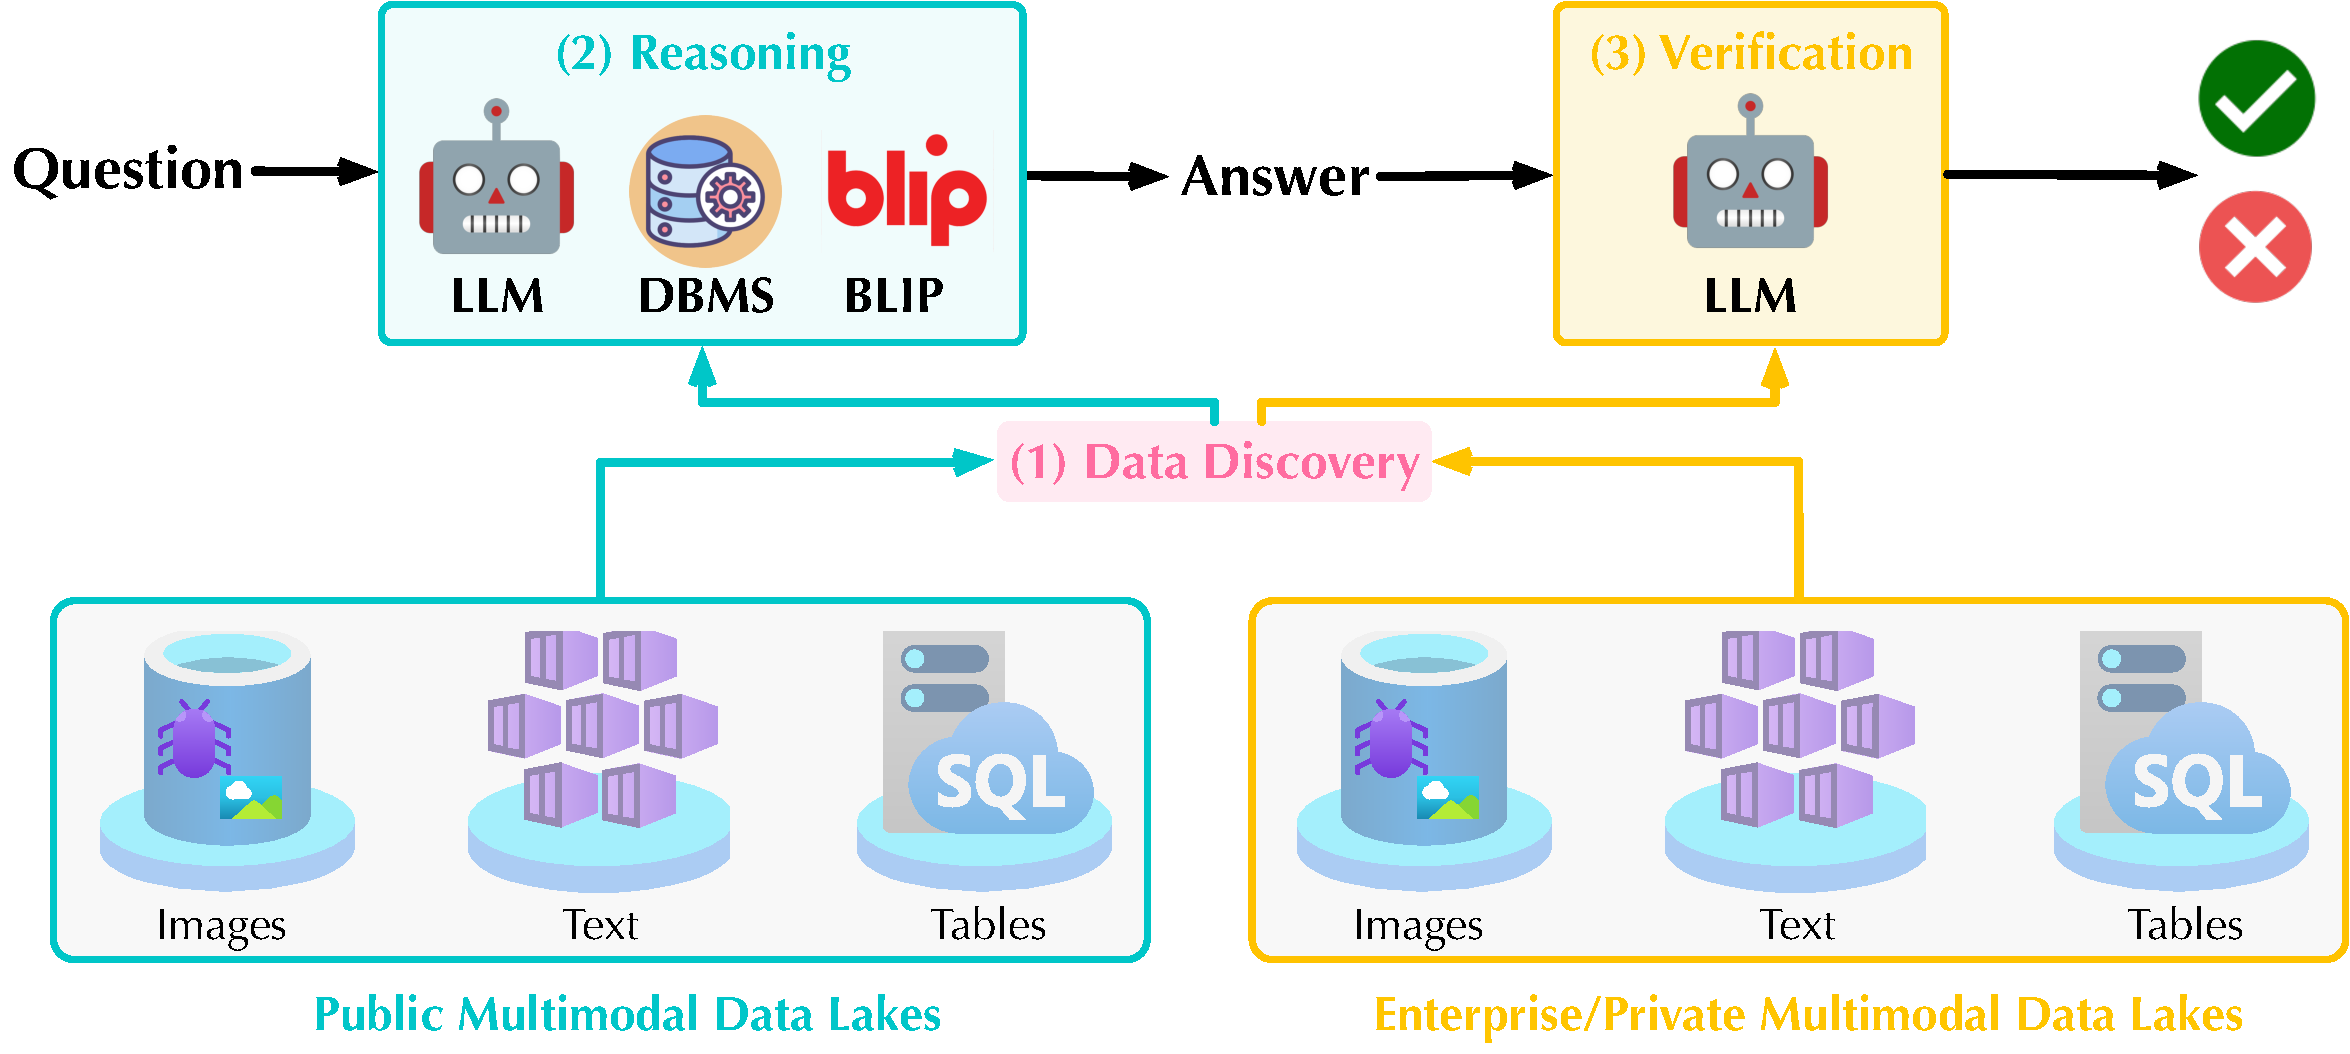
\includegraphics[width=\textwidth]{submissions/Nan2024/figs/mot}
\end{center}
\vspace{-2em}
\caption{An Overview of \sys.}
\label{fig:symphony}
\vspace{-1em}
\end{figure}

% Even with RAG-based reasoning, errors may still occur due to the probabilistic nature of generative models. To mitigate this, \sys includes a RAG-powered verification module. After generating an answer, \sys can retrieve (new) relevant data from more reliable data lakes to verify the output for correctness and consistency. This process ensures that the answer aligns with trusted sources, and private or enterprise-specific data lakes can be optionally utilized, offering domain-specific data that ensures the answer meets user expectations and specific requirements. %(Section~\ref{sec:verifai})

\stitle{Roadmap.}
Section~\ref{sec:learning} describes the \discovery module.
Section~\ref{sec:reasoning} discusses the \reason module.
Section~\ref{sec:verifai} presents the \verify module.
Section~\ref{sec:exp} describes empirical findings.
Section~\ref{sec:open} identifies open problems.
Section~\ref{sec:related} discusses related work.
Finally, we close this paper by concluding remarks in Section~\ref{sec:conclusion}.